\documentclass[border=3pt]{standalone}
\usepackage[T1]{fontenc}
\usepackage{lmodern}
\usepackage{amsmath,amssymb}
\usepackage{tikz}
\usepackage{pgfplots}
\pgfplotsset{compat=1.17}
\usepgfplotslibrary{groupplots}
\usetikzlibrary{arrows.meta,calc,positioning,fit,backgrounds}

% Multi-camera surveillance: local tracking in every camera, identity matching on a central server.
\newcommand{\camicon}[1]{%
  \begin{scope}[shift={#1}]
    \fill[black!70, rounded corners=0.6pt] (0,0) rectangle (0.56,0.26);
    \fill[black!70] (0.56,0.05) -- (0.74,-0.03) -- (0.74,0.29) -- (0.56,0.21) -- cycle;
    \draw[black!70, line width=1.2pt] (0.16,0) -- (0.16,-0.14) -- (-0.02,-0.14);
  \end{scope}}
\newcommand{\person}[2]{%
  \begin{scope}[shift={#1}, scale=#2]
    \fill[black!70] (0,0.62) circle (0.11);
    \fill[black!70, rounded corners=1.5pt] (-0.13,0.15) rectangle (0.13,0.48);
    \fill[black!70] (-0.11,0.18) rectangle (-0.02,-0.12);
    \fill[black!70] (0.02,0.18) rectangle (0.11,-0.12);
  \end{scope}}
\begin{document}
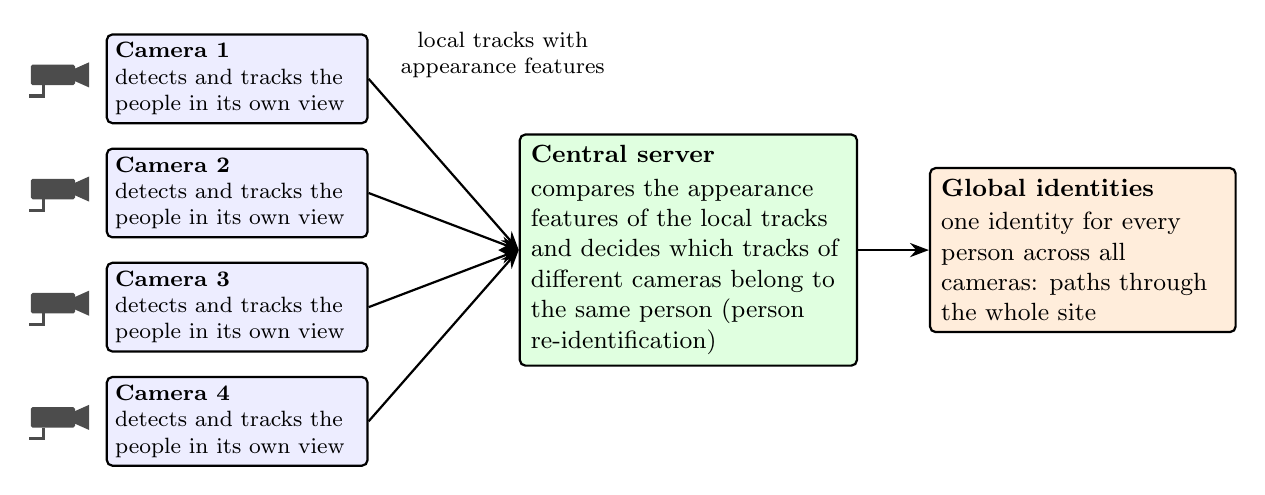
\begin{tikzpicture}[
  font=\small,
  cam/.style={draw, thick, rounded corners=2pt, fill=blue!7, align=flush left, text width=31mm,
              inner sep=3pt, font=\footnotesize, minimum height=11mm},
  proc/.style={draw, thick, rounded corners=2pt, fill=green!12, align=flush left, text width=40mm, inner sep=4pt},
  res/.style={draw, thick, rounded corners=2pt, fill=orange!14, align=flush left, text width=36mm, inner sep=4pt},
  arr/.style={-{Stealth[length=2.4mm]}, thick},
  lab/.style={font=\footnotesize, fill=white, inner sep=1.5pt, align=center}]
\foreach \k/\y in {1/0, 2/-1.45, 3/-2.9, 4/-4.35} {
  \node[cam, anchor=west] (c\k) at (1.0,\y) {\textbf{Camera \k}\\ detects and tracks the\\ people in its own view};
  \camicon{(0.05,\y-0.08)}
}
\node[proc] (srv) at (8.4,-2.175) {\textbf{Central server}\\[1pt]
  compares the appearance features of the local tracks and decides which tracks of
  different cameras belong to the same person (person re-identification)};
\node[res, right=9mm of srv] (id) {\textbf{Global identities}\\[1pt] one identity for every person
  across all cameras: paths through the whole site};
\foreach \k in {1,2,3,4} \draw[arr] (c\k.east) -- (srv.west);
\node[lab, anchor=south] at ($(c1.east)!0.5!(srv.north west)+(0.75,0.3)$) {local tracks with\\ appearance features};
\draw[arr] (srv) -- (id);
\end{tikzpicture}
\end{document}
